% Multiple Choice Question 31 to 33 (3 questions)

\textbf{See the instruction for questions \inteval{\value{question}+1} to \inteval{\value{question}+3}.} 

\begin{center}
    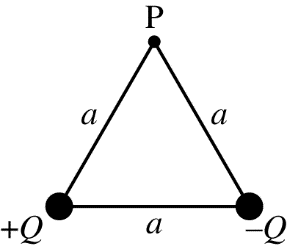
\includegraphics[scale=0.3]{images/img-015-031.png}
\end{center}
    
Two small spheres have charges $+Q$ and $-Q$ and are located at the bottom corners of an equilateral triangle, as shown in the figure above. The equilateral triangle has sides of length $a$, and point P is at the top corner of the triangle.

% Multiple Choice Question 31
\begin{questions}\setcounter{question}{30}\question
The potential energy stored in the charge configuration shown is

\begin{oneparchoices}
    \choice $\dfrac{Q^{2}}{4 \pi \varepsilon_{0} a}$
    \choice $\dfrac{Q}{4 \pi \varepsilon_{0} a^{2}}$
    \choice Zero
    \choice $-\dfrac{Q}{4 \pi \varepsilon_{0} a^{2}}$ 
    \choice $-\dfrac{Q^{2}}{4 \pi \varepsilon_{0} a}$
\end{oneparchoices}
\end{questions}

% Multiple Choice Question 32
\begin{questions}\setcounter{question}{31}\question
The electric potential at point $P$ due to the two spheres is

\begin{oneparchoices}
    \choice Zero
    \choice $\dfrac{Q}{4 \pi \varepsilon_{0} a}$
    \choice $\dfrac{Q}{4 \pi \varepsilon_{0} a^{2}}$
    \choice $\dfrac{2 Q}{4 \pi \varepsilon_{0} a}$
    \choice $\dfrac{2 Q}{4 \pi \varepsilon_{0} a^{2}}$
\end{oneparchoices}
\end{questions}

% Multiple Choice Question 33
\begin{questions}\setcounter{question}{32}\question
The direction of the electric field at point P due to the two spheres is

\begin{choices}
    \choice to the left
    \choice to the right
    \choice toward the bottom of the page
    \choice toward the top of the page
    \choice undefined, because the magnitude of the electric field at point P is zero
\end{choices}
\end{questions}
